\section{\method{} Design}

\subsection{Overview}

\begin{figure}
    % [ht]
    \centering
    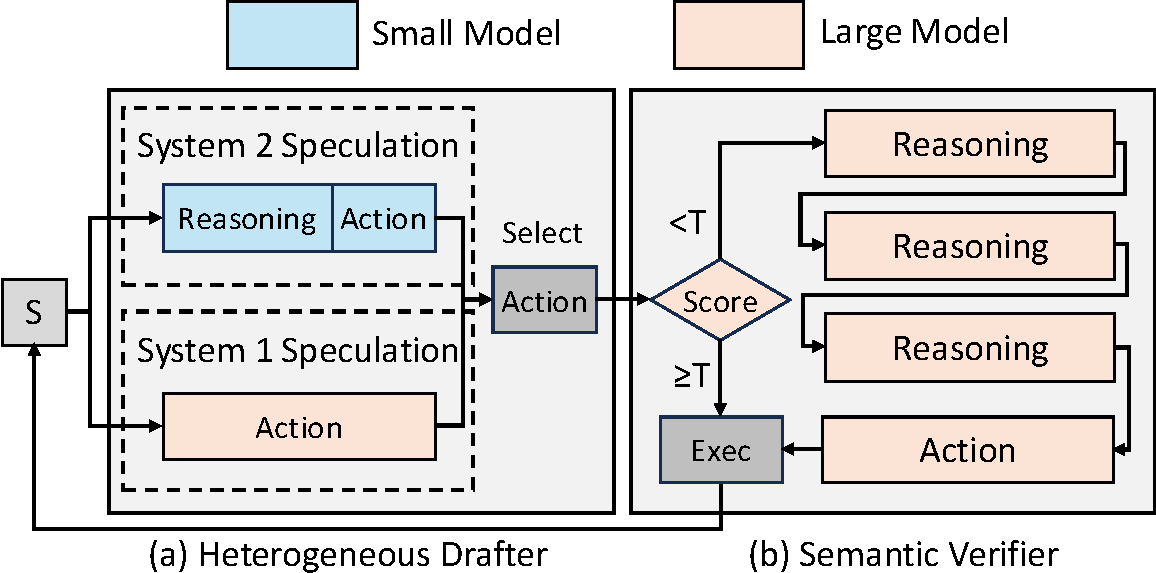
\includegraphics[width=\linewidth]{figs/overview.pdf}
    \caption{Overview of \method{}. 
    %  as an action-level speculative framework with heterogeneous drafting and semantic verification.
     }
    \label{fig:overview}
\end{figure}

We propose \method{}, a dual-process speculative framework for deep research agents.
The core design principle of \method{} is to allocate inference resources \emph{heterogeneously} across actions for high speculation accuracy, while preserving end-to-end agent performance through lightweight, step-wise semantic verification.

As illustrated in Figure~\ref{fig:overview}, \method{} follows a draft--verify workflow.
At each decision step, \method{} generates two candidate actions in parallel:
(i) a \textit{System~2} draft produced by a small model with explicit reasoning, and
(ii) a \textit{System~1} draft via a large model skipping reasoning.
The framework then selects a provisional draft based on the action type and the reasoning footprint from the small-model output.
Finally, the selected draft is evaluated by a semantic verifier using a full-capacity base model.
Drafts judged to be semantically consistent with the current reasoning trajectory are accepted and executed directly; otherwise, \method{} falls back to full-capacity reasoning to regenerate the action.

% Motivated by the observations and analysis, we propose \method{}, a dual-process speculative framework for deep research agents.
% \method{} is designed to allocate inference resources heterogeneously across actions while maintaining end-to-end accuracy through lightweight verification.

% As illustrated in Figure~\ref{fig:overview}, \method{} follows a draft--verify workflow.
% At each step, \method{} drafts two candidate actions in parallel: a \textit{System~2} draft from the small model with reasoning, and a \textit{System~1} draft from the large model without reasoning; it then selects between them using the action type and the draft’s reasoning footprint.
% The drafted action is then evaluated by a semantic verifier implemented with a full-capacity model.
% Actions that are judged to be consistent with the current reasoning trajectory are accepted and executed directly, whereas low-quality drafts trigger fallback to full-capacity reasoning.

\subsection{Heterogeneous Draft}
\label{subsec:hetero_draft}

% \method{} implements heterogeneous drafting by generating two candidate actions at each step and selecting the one that best matches the inference demand of the current decision.
% Given the current state $s_t$, we produce:
% (i) a \textit{System~2} draft $(z_s, a_s)$ using the small model with explicit reasoning, and
% (ii) a \textit{System~1} draft $a_l$ using the large model without explicit reasoning.
% The key question is how to select the final drafted action while preserving useful reasoning context.

\method{} implements heterogeneous drafting by producing two candidate actions at each step and adaptively selecting the one that best matches the inference demand of the current decision.
Formally, given the current state $s_t$, we generate a System~2 draft $(z_s, a_s)$ using SLM and
a System~1 draft $a_l$ using LLM.
The key question is how to select the final drafted action while retaining reasoning information that is valuable for long-horizon planning.


% We use the action type produced by the small-model draft as the primary routing signal.
% If the small model proposes a \textsc{Search} action, we keep $a_s$ as the draft action, since \textsc{Search} benefits from explicit reasoning and the small model is sufficient when paired with reasoning.
% If the small model proposes a \textsc{Visit} action, we typically replace it with the large-model no-reasoning draft $a_l$, since \textsc{Visit} relies more on the large model’s parametric capacity for direct decisions on concrete inputs.
\paragraph{Action-aware selection.}
We use the action type predicted by the small-model draft as the primary routing signal.
If the small model generates a Search action, we retain $a_s$ as the draft action, as Search typically benefits from explicit reasoning and can be reliably handled by a smaller model when paired with a reasoning trace.
If the small model proposes a Visit action, we instead select the large-model draft $a_l$ in most cases, since Visit actions rely more heavily on the large model's parametric capacity to make direct decisions on concrete inputs.

\paragraph{Preserving long-horizon reasoning.}
An important exception arises when the small-model draft produces a long reasoning trace before emitting its action.
Empirically, such extended reasoning often contains global analysis or intermediate summaries that remain useful beyond the current step, regardless of whether the final action is Search or Visit.
To preserve this information, when the length of the small-model reasoning exceeds a threshold $\tau_{\text{think}}$, we choose the full draft $(z_s, a_s)$ even if the action type is Visit.
This mechanism ensures that high-level reasoning is not discarded when it may benefit subsequent decisions.


\subsection{Semantic Verification}
\label{subsec:semantic_verification}


To maintain end-to-end accuracy, \method{} performs lightweight semantic verification at every step.
Instead of enforcing action-level matching, the verifier assesses whether the drafted reasoning and action are likely to make meaningful progress.
This design is motivated by the observation that intermediate agent decisions are often tolerant to approximation as illustrated in table~\ref{tab:action}.
Moreover, this approach avoids the reasoning delays from the base models to generate actions, enabling faster verification.   

Given the current state $s_t$ and a draft consisting of an optional reasoning trace $z_t$ and a candidate action $a_t$, we query the large model as a critic and ask it to answer \texttt{Yes} or \texttt{No}.
The prompt instructs the critic to jointly assess (i) whether the reasoning is coherent (if present) and (ii) whether the proposed action is useful for making progress.
The exact prompt template is provided in Appendix~\ref{app:verifier_prompt}.

Although the critic produces a discrete verdict, a \emph{continuous} signal is necessary to trade off speed and reliability.
We therefore convert the critic's output distribution into a real-valued confidence score.

Let $p_{\mathrm{acc}}(s_t,z_t,a_t)$ and $p_{\mathrm{rej}}(s_t,z_t,a_t)$ denote the critic's probabilities of answering \texttt{Yes} and \texttt{No}, respectively.
We define the verification score as the log-probability margin:
\begin{equation}
\mathrm{score}(s_t, z_t, a_t)
=
\log p_{\mathrm{acc}}(s_t, z_t, a_t)
-
\log p_{\mathrm{rej}}(s_t, z_t, a_t),
\label{eq:verifier_score}
\end{equation}
which corresponds to the log-odds of acceptance and provides a stable, monotonic measure of verifier confidence.

We accept the draft if its score exceeds a threshold $\tau$:
\begin{equation}
\textsc{Accept}(z_t, a_t)
\quad \text{if} \quad
\mathrm{score}(s_t, z_t, a_t) \ge \tau,
\label{eq:accept_rule}
\end{equation}
and otherwise trigger fallback.
Fallback regenerates the step using the full-capacity model with explicit reasoning and continues execution with the regenerated action.
This verification-and-fallback procedure follows a standard speculative pattern: propose a fast approximate step, validate it with a stronger critic, and only pay the cost of full reasoning when the draft is unlikely to be reliable.

Since the score scale depends on the critic model, we select $\tau$ offline on a held-out development set.
We sweep candidate thresholds and choose a fixed $\tau$ that preserves end-to-end accuracy while maximizing the acceptance rate, and keep it fixed at runtime.
This allows \method{} to allocate expensive full-capacity reasoning only to the minority of uncertain steps, improving overall time-to-solution. Additional empirical evidence on the effectiveness of this verifier score is provided in Appendix~\ref{app:verifier_scores}.




\iffalse

Motivated by the observations and analysis, we propose \method{}, a dual-process speculative framework for deep research agents.
\method{} is designed to allocate inference resources heterogeneously across actions while maintaining end-to-end accuracy through lightweight verification.

As illustrated in Figure~\ref{fig:overview}, \method{} follows a draft--verify workflow.
At each step, \method{} drafts two candidate actions in parallel: a \textit{System~2} draft from the small model with reasoning, and a \textit{System~1} draft from the large model without reasoning; it then selects between them using the action type and the draft’s reasoning footprint.
The drafted action is then evaluated by a semantic verifier implemented with a full-capacity model.
Actions that are judged to be consistent with the current reasoning trajectory are accepted and executed directly, whereas low-quality drafts trigger fallback to full-capacity reasoning.

\subsection{Heterogeneous Draft}
\label{subsec:hetero_draft}

\method{} implements heterogeneous drafting by generating two candidate actions at each step and selecting the one that best matches the inference demand of the current decision.
Given the current state $s_t$, we produce:
(i) a \textit{System~2} draft $(z_s, a_s)$ using the small model with explicit reasoning, and
(ii) a \textit{System~1} draft $a_l$ using the large model without explicit reasoning.
The key question is how to select the final drafted action while preserving useful reasoning context.

\paragraph{Action-aware selection.}
We use the action type produced by the small-model draft as the primary routing signal.
If the small model proposes a \textsc{Search} action, we keep $a_s$ as the draft action, since \textsc{Search} benefits from explicit reasoning and the small model is sufficient when paired with reasoning.
If the small model proposes a \textsc{Visit} action, we typically replace it with the large-model no-reasoning draft $a_l$, since \textsc{Visit} relies more on the large model’s parametric capacity for direct decisions on concrete inputs.

\paragraph{Preserving long-horizon reasoning.}
A subtle but important case arises when the small-model draft generates a long reasoning trace before emitting its action.
In practice, such long reasoning often contains global analysis or intermediate summaries that are useful for subsequent steps, regardless of whether the final action is \textsc{Search} or \textsc{Visit}.
Therefore, when the small-model reasoning length exceeds a threshold $\tau_{\text{think}}$, we preserve its reasoning trace even if the action type is \textsc{Visit}.
Concretely, we keep $(z_s, a_s)$ as the drafted output in this case, so that the accumulated context retains the small model’s high-level reasoning.


\subsection{Semantic Verification}
\label{subsec:semantic_verification}

 \method{} performs lightweight semantic verification at every step to preserve end-to-end accuracy.
Instead of enforcing strict action-level equivalence, the verifier checks whether the drafted reasoning and action are semantically consistent with the current trajectory and are likely to provide useful progress.
This follows the observation that intermediate decisions are tolerant to approximation as long as their semantic contribution is preserved, and that a strong model can efficiently assess such intermediate steps and trigger correction only when necessary.

Given the current state $s_t$ and a draft output consisting of an optional reasoning trace $z_t$ and a candidate action $a_t$, we query the full-size model as a critic to output a single binary judgment (\texttt{Yes} or \texttt{No}).
The prompt asks the critic to jointly assess whether the reasoning is consistent and whether the action is useful for progress.
When the draft pathway skips explicit reasoning, we set $z_t=\emptyset$.
We provide the exact prompt template in Appendix~\ref{app:verifier_prompt}.

Although the output is binary, the critic assigns probabilities to both acceptance and rejection.
We therefore derive a continuous verification score from the model distribution.
Let $p_{\mathrm{v}}(\cdot \mid s_t, z_t, a_t)$ denote the next-token distribution under the verifier prompt.
To ensure robustness to minor formatting and tokenizer variability, we aggregate probability mass over semantically equivalent affirmative and negative responses.
We define the verification score as the log-probability margin:
\begin{equation}
\mathrm{score}(s_t, z_t, a_t)
=
\log p_{\mathrm{acc}}(s_t, z_t, a_t)
-
\log p_{\mathrm{rej}}(s_t, z_t, a_t),
\label{eq:verifier_score}
\end{equation}
where $p_{\mathrm{acc}}$ and $p_{\mathrm{rej}}$ are the aggregated probabilities of affirmative and negative responses, respectively.


\paragraph{Acceptance rule and fallback.}
We accept the drafted output when its score exceeds a threshold $\tau$:
\begin{equation}
\textsc{Accept}(z_t, a_t)
\quad \text{if} \quad
\mathrm{score}(s_t, z_t, a_t) \ge \tau,
\label{eq:accept_rule}
\end{equation}
and otherwise trigger fallback.
Fallback regenerates the step using the full-size model with explicit reasoning and continues execution with the regenerated action.
This verification-as-scoring mechanism matches the speculative reasoning pattern of proposing an approximate step using a lightweight pathway, assessing it with a stronger model, and correcting it only when needed.

\paragraph{Threshold profiling.}
The score scale depends on the verifier model and tokenizer, so $\tau$ is model-dependent.
We therefore profile $\tau$ offline for each model pair on a held-out development set.
Concretely, we sweep candidate thresholds and choose a fixed $\tau$ that preserves end-to-end accuracy while maximizing acceptance rate, and keep $\tau$ fixed at runtime.
This allows \method{} to concentrate expensive full-capacity reasoning on the minority of steps where the draft is unlikely to be reliable, improving end-to-end time-to-solution.

\fi